\documentclass{article}
\usepackage{tikz}
\usepackage{amsmath}
\usepackage{caption}
\usepackage{float}
\usepackage{graphicx}
\usepackage{hyperref}
\usepackage{listings}
\usepackage{xcolor}
\usepackage{tikz}
\usetikzlibrary{arrows.meta, positioning}

\renewcommand{\thesubsection}{\arabic{subsection}}
\definecolor{codebg}{RGB}{248,248,248}
\definecolor{keywordcolor}{RGB}{0,0,180}
\definecolor{stringcolor}{RGB}{163,21,21}
\definecolor{commentcolor}{RGB}{0,128,0}
\definecolor{numbercolor}{RGB}{128,0,128}
\definecolor{decoratorcolor}{RGB}{200,100,0}

\lstdefinestyle{py}{
  language=Python,
  backgroundcolor=\color{codebg},
  basicstyle=\ttfamily\small,
  keywordstyle=\color{keywordcolor}\bfseries,
  stringstyle=\color{stringcolor},
  commentstyle=\color{commentcolor}\itshape,
  numberstyle=\tiny\color{gray},
  numbers=left,
  stepnumber=1,
  numbersep=8pt,
  showstringspaces=false,
  breaklines=true,
  frame=single,
  rulecolor=\color{black!30},
  tabsize=2,
  morekeywords={self},
}
\hypersetup{
            pdfauthor={Xavier Sebastian A}, 
            pdftitle={Compsci:790-HW3}, 
            pdfsubject={HW3}, 
            pdfkeywords={GPU,Triton,JAX,Pallas,Kernal Fusion,JIT},
            pdfproducer={LaTeX with hyperref},
            pdfcreator={pdflatex},
            pdfborder={0 0 0}, 
            pdfstartview=FitH
        }

\title{Homework 3}
\author{Xavier Sebastian A}
%\date{\today}

\begin{document}

\maketitle
\section{Conceptual Questions}
\subsection{Explain the difference between tracing-based and scripting-
based JIT compilation. Give a concrete example of a Python function
that would work correctly with scripting but fail with tracing}
\subsubsection*{Answer:}
Tracing-based JIT runs the function once and records the operations that happen during that execution. 
It builds a computation graph based on that single run. 
Because of this, it cannot correctly handle control flow that depends on input values.

Scripting-based JIT analyses the program code directly and converts it into an intermediate representation. 
Since it understands the structure of the code, it can correctly handle conditions, loops, and other control flow statements.
The following example demonstrates scripting-based compilation in PyTorch \cite{jit_compilation_ml}:

\begin{lstlisting}[style=py]
@torch.jit.script # Example decorator
def conditional_op(x, threshold):
  # Scripting compiler parses this structure
  if x.sum() > threshold:
    result = x * 2
  else:
    result = x + 1
  return result
\end{lstlisting}
Tracing may record only one branch of the if statement depending on the input used during tracing. 
If the condition later changes, the result may become incorrect. 
Scripting works correctly because it keeps both branches in the compiled graph.

\subsection{Consider the following JAX function:}
\begin{lstlisting}[style=py]
@jax.jit
def process_batch(data, batch_size):
    num_batches = data.shape[0] // batch_size
    results = []
    for i in range(num_batches):
        batch = data[i * batch_size:(i + 1) * batch_size]
        results.append(jnp.sum(batch ** 2))
    return jnp.array(results)
\end{lstlisting}
What potential performance issue might arise with this JIT-compiled function? How would you fix it?
\subsubsection*{Answer:}
The function creates a Python list and appends values inside a loop. 
Python loops and list operations reduce the efficiency of JAX because they prevent proper optimisation during compilation.
JAX works best when operations are written in a vectorised form using array operations. 
A better solution is to reshape the data and compute the result using built in array functions.
Fixed version:
\begin{lstlisting}[style=py]
@jax.jit
def process_batch(data, batch_size):
    num_batches = data.shape[0] // batch_size
    data = data[:num_batches * batch_size]
    data = data.reshape(num_batches, batch_size)
    return jnp.sum(data ** 2, axis=1)
\end{lstlisting}
This removes the Python loop and allows JAX to perform faster compiled execution.

\subsection{The lecture mentioned that operator fusion can reduce memory traffic. 
For the expression $y = \sin(\cos(x)) + \exp(x)$ calculate:}

\begin{enumerate}
\item[(a)] The number of GPU kernel launches and global memory
reads/writes in eager mode (assume each operation reads inputs from
global memory and writes outputs to global memory).

\item[(b)] The number in fused mode (one kernel, intermediate values
stored in registers).

\item[(c)] The theoretical memory bandwidth reduction factor.
\end{enumerate}

\subsubsection*{Answer:}
\begin{enumerate}
    \item [(a)]
    Each operation runs as a separate GPU kernel.
    Operations performed:
    \begin{itemize}
    \item $\cos(x)$
    \item $\sin(\cdot)$
    \item $\exp(x)$
    \item addition
    \end{itemize}
    Total kernel launches $= 4$.Each operation reads data from global memory and writes the results back to global memory.

\item[(b)]
All operations are combined into a single GPU kernel.Total kernel launches $= 1$.Intermediate values remain inside GPU registers instead of being written to global memory.

\item[(c)]
In eager execution there are roughly $8$ memory operations ($4$ reads and $4$ writes).In fused execution there are $2$ memory operations ($1$ read and $1$ write).
Therefore, the theoretical reduction factor is $\frac{8}{2} = 4$.So the memory traffic is reduced by approximately four times.
\end{enumerate}

\subsection{Why does dynamic control flow (e.g., if statements depending
on tensor values) pose a challenge for JIT compilation? Explain both the
JAX and PyTorch approaches to handling this.}


\subsubsection*{Answer:}

Dynamic control flow occurs when program execution depends on values that are known only at runtime. JIT compilers typically construct a static computation graph before execution. If the program contains branches that depend on runtime tensor values, the compiler cannot determine the correct execution path during compilation.

JAX addresses this issue by providing specialised control-flow primitives such as \texttt{lax.cond}, \texttt{lax.scan}, and \texttt{lax.while\_loop}. These primitives explicitly represent control flow within the compiled graph.

PyTorch addresses the issue using \texttt{TorchDynamo}, which traces Python execution and captures graph segments dynamically. When unsupported control flow appears, the system may partially compile the program or fall back to eager execution.

\subsection{When you run \texttt{torch.compile} on a function for the first time,
it’s slower than the eager version. Why? What specific steps happen
during this first call that don’t happen in subsequent calls?}

\subsubsection*{Answer:}

The first execution of a function compiled with \texttt{torch.compile} involves several additional steps before the program runs.

During the first call:

\begin{itemize}
\item \texttt{TorchDynamo} traces the Python function and extracts a computation graph.
\item The graph is analysed and optimised.
\item \texttt{TorchInductor} or another backend compiler generates optimised kernels.
\item The generated code is compiled for the target hardware.
\item The compiled graph is cached for reuse.
\end{itemize}

These compilation steps introduce overhead during the first execution. Later executions reuse the cached compiled graph and therefore run significantly faster.

\section{Programming: JAX JIT Deep Dive}

\subsection{Part 1: Measuring Compilation Overhead}

In this experiment we measured the runtime of a function performing several elementwise operations on matrices of different sizes. Three cases were evaluated: eager execution (without JIT), the first call with JIT compilation, and the second call using the cached compiled function.

The first JIT call is slower because JAX must trace the function and compile it using XLA. This compilation step introduces overhead. However, the second JIT call reuses the compiled program and therefore runs significantly faster.

As the matrix size increases, eager execution becomes slower because each operation is executed individually. JIT compilation improves performance because the compiled program optimises the sequence of operations and reduces interpreter overhead.

\begin{figure}[H]
\centering
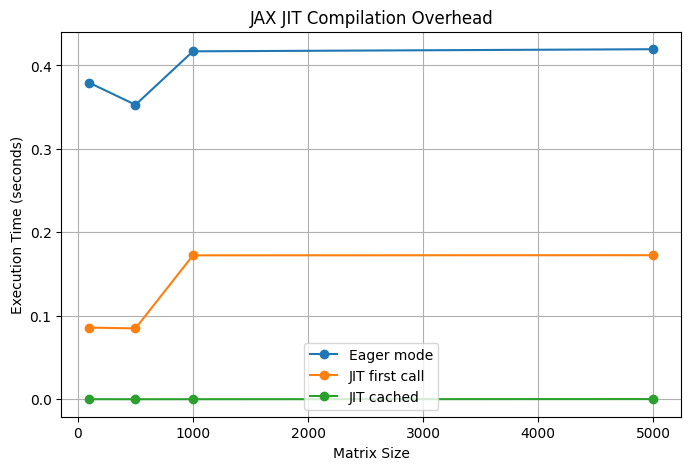
\includegraphics[width=0.75\linewidth]{jit1.png}
\caption{Execution time comparison between eager execution, first JIT call, and second JIT call for different matrix sizes.}
\end{figure}


\subsection{Part 2: Shape Specialization}

In this part we analysed how JAX handles inputs with different tensor shapes. A JIT compiled function computing the mean of each row was executed with multiple input shapes.

Using \texttt{jax.make\_jaxpr}, we observed that JAX retraces the computation when the input tensor shape changes. When the same shape is used again, the previously compiled program is reused.

This behaviour is called \textbf{shape specialization}. JAX generates optimised machine code specific to each input shape. When a new shape appears, the compiler must retrace and generate a new compiled version of the function.

The timing results show that calls with previously seen shapes execute faster, while calls with new shapes include additional compilation overhead.

\begin{figure}[H]
\centering
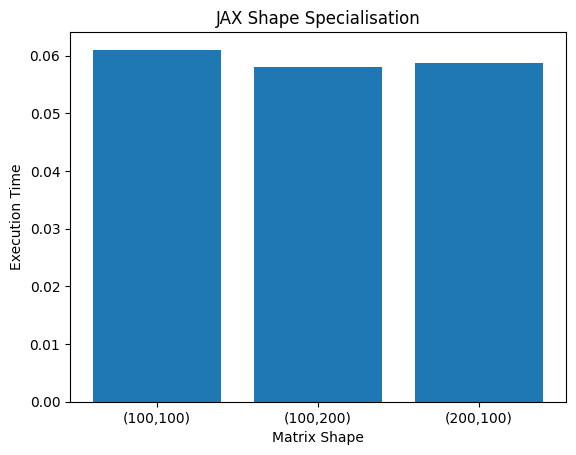
\includegraphics[width=0.7\linewidth]{jax1.png}
\caption{Execution time for different input shapes demonstrating retracing behaviour.}
\end{figure}


\subsection{Part 3: Operator Fusion Analysis}

This experiment evaluates the benefits of operator fusion using JIT compilation. The function
$f(x) = \sum_{i=1}^{100} (\sin^i(x) + \cos^i(x))$was implemented using two approaches.

In the eager version, each elementwise operation (sine, cosine, and addition) is executed independently. This leads to a large number of individual operations and higher kernel launch overhead.

In the JIT compiled version, the XLA compiler analyses the computation graph and performs \textbf{operator fusion}. Multiple elementwise operations are combined into fewer execution kernels. This reduces kernel launch overhead and improves memory efficiency.

The measured runtime shows a significant performance improvement for the JIT version. The speedup occurs because the compiler executes many operations together instead of launching separate kernels for each operation.

The theoretical number of operations is approximately 10,200 elementwise operations (5050 sine operations, 5050 cosine operations, and around 100 additions). In eager execution these operations may launch many kernels, whereas the JIT compiled version fuses them into fewer kernels.

The measured execution times show that the JIT compiled version achieves a much faster runtime due to reduced overhead and improved memory locality.

\section{Programming: PyTorch compile Analysis}
\subsection{Part 1: Comparing Backends}

In this experiment we compared different compilation backends supported by \texttt{torch.compile}. A simple neural network with three linear layers and ReLU activations was executed using the following backends:

\begin{itemize}
\item eager
\item aot\_eager
\item inductor
\item cudagraphs
\end{itemize}

The eager backend executes operations directly without compilation. The aot\_eager backend traces the computation graph but still runs operations using eager kernels. The inductor backend performs aggressive compilation and optimisation to generate fused kernels. The cudagraphs backend records the execution graph and reduces kernel launch overhead.

The performance results show that different backends have different runtime behaviour due to their compilation strategies. Compilation overhead can make some backends slower for small workloads, while optimised backends provide better performance for repeated execution.

\begin{figure}[H]
\centering
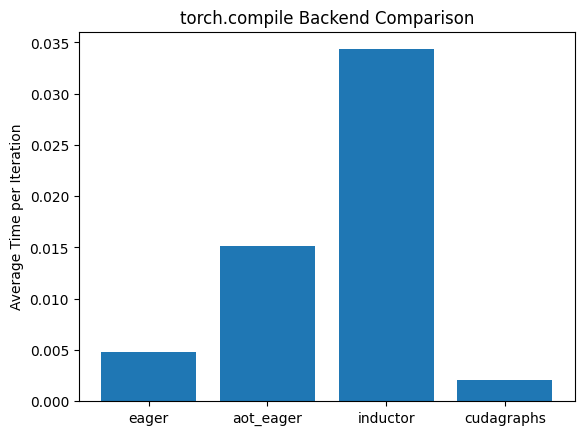
\includegraphics[width=0.7\linewidth]{be1.png}
\caption{Average runtime comparison for different torch.compile backends.}
\end{figure}


\subsection{Part 2: Debugging Compilation Failures}

Some Python constructs cannot be efficiently compiled by \texttt{torch.compile}. We tested several problematic functions to analyse compilation failures.

The first example used a Python conditional statement depending on a tensor value. TorchDynamo reported a graph break because tensor-dependent control flow cannot be directly traced into a static computation graph.

The second example used a Python dictionary to store tensor values. Python data structures are not part of tensor computation graphs, which results in graph breaks.

The third example used a Python loop performing repeated exponentiation operations. Although this function can be compiled, the loop structure leads to suboptimal performance because the compiler cannot fully optimise repeated operations.

Using \texttt{torch.dynamo.explain()}, we identified graph breaks and debugging information describing why compilation failed or was inefficient. By rewriting the functions using tensor operations and removing Python side effects, the compiler was able to successfully capture the computation graph and execute the code more efficiently.


\subsection{Part 3: Graph Capture and Inspection}

To analyse graph capture behaviour, we created a function performing two matrix multiplications, a ReLU activation, a residual addition, and layer normalization. The function also included a Python print statement and a list modification.

Using \texttt{torch.dynamo.explain()}, we observed that tensor operations such as matrix multiplication, ReLU activation, addition, and layer normalization were captured in the computation graph.

However, Python side-effect operations such as \texttt{print()} and list modification were not included in the graph. TorchDynamo cannot represent these operations as tensor computations, so they are executed outside the compiled graph.

The resulting computation graph therefore contains only the tensor operations required for numerical computation.

\begin{figure}[H]
\centering
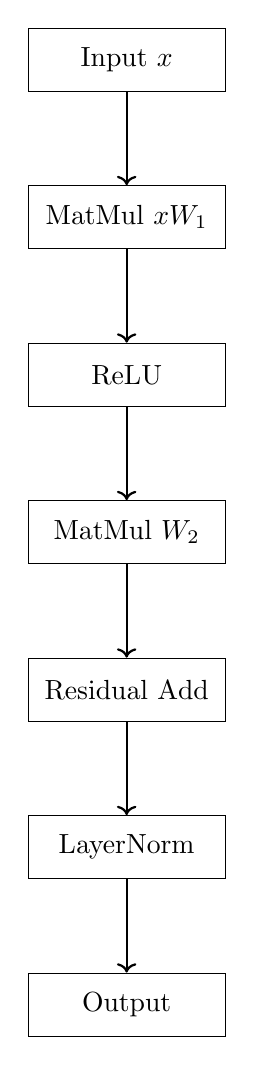
\begin{tikzpicture}[
node distance=2cm,
box/.style={rectangle, draw, minimum width=2.5cm, minimum height=0.8cm},
arrow/.style={->, thick}
]

\node[box] (input) {Input $x$};
\node[box, below of=input] (mat1) {MatMul $xW_1$};
\node[box, below of=mat1] (relu) {ReLU};
\node[box, below of=relu] (mat2) {MatMul $W_2$};
\node[box, below of=mat2] (add) {Residual Add};
\node[box, below of=add] (norm) {LayerNorm};
\node[box, below of=norm] (output) {Output};

\draw[arrow] (input) -- (mat1);
\draw[arrow] (mat1) -- (relu);
\draw[arrow] (relu) -- (mat2);
\draw[arrow] (mat2) -- (add);
\draw[arrow] (add) -- (norm);
\draw[arrow] (norm) -- (output);

\end{tikzpicture}
\caption{Captured computation graph from \texttt{torch.compile}.}
\end{figure}

\section*{Code Repository}

Project repository:  
\url{https://github.com/xavier-s-a/hw3-790}

\begin{thebibliography}{9}

\bibitem{jit_compilation_ml}
JIT Tracing vs Scripting
\textit{Tracing vs. Scripting Approaches.}  
\url{https://apxml.com/courses/compiler-runtime-optimization-ml/chapter-7-jit-compilation-ml/jit-tracing-vs-scripting}



\end{thebibliography}
\end{document}

